\documentclass[12pt,a4paper]{report}

\usepackage{fontspec}
\setmainfont{Times New Roman}

\usepackage[vietnamese]{babel}
\usepackage[top=3.5cm, bottom=3.0cm, left=3.5cm, right=2.0cm]{geometry}
\usepackage{setspace}
\onehalfspacing

\usepackage{graphicx}
\usepackage{booktabs}
\usepackage{tabularx}
\usepackage{longtable}
\usepackage{multirow}
\usepackage{amsmath,amssymb}
\usepackage{caption}
\captionsetup[table]{skip=6pt}
\captionsetup[figure]{skip=6pt}
\usepackage{float}
\usepackage{enumitem}
\usepackage{fancyhdr}
\usepackage{xurl}
\usepackage[colorlinks=true,linkcolor=black,citecolor=black,urlcolor=blue]{hyperref}
\usepackage{titlesec}
\usepackage{tikz}

% Định dạng tiêu đề theo mẫu chuẩn Phenikaa
\titleformat{\chapter}[hang]{\normalfont\Large\bfseries}{\thechapter}{1em}{\MakeUppercase}
\titlespacing*{\chapter}{0pt}{-0.5cm}{1.2em}
\titleformat{\section}[hang]{\normalfont\large\bfseries}{\thesection}{1em}{}
\titlespacing*{\section}{0pt}{1.2ex plus .5ex minus .2ex}{0.8ex}
\titleformat{\subsection}[hang]{\normalfont\normalsize\bfseries}{\thesubsection}{1em}{}
\titlespacing*{\subsection}{0pt}{1.0ex plus .4ex minus .2ex}{0.6ex}

\setlength{\headheight}{15pt}
\setlength{\parindent}{18pt}
\setlength{\parskip}{0pt}

% Đầu trang và chân trang
\pagestyle{fancy}
\fancyhf{}
\fancyhead[L]{\small\textit{Báo cáo học phần Xử lý ngôn ngữ tự nhiên}}
\fancyfoot[L]{\small\textit{Phân loại tin thật và tin giả tiếng Việt}}
\fancyfoot[R]{\small\thepage}
\renewcommand{\headrulewidth}{0.8pt}
\renewcommand{\footrulewidth}{0.8pt}

\fancypagestyle{plain}{
  \fancyhf{}
  \fancyhead[L]{\small\textit{Báo cáo học phần Xử lý ngôn ngữ tự nhiên}}
  \fancyfoot[L]{\small\textit{Phân loại tin thật và tin giả tiếng Việt}}
  \fancyfoot[R]{\small\thepage}
  \renewcommand{\headrulewidth}{0.8pt}
  \renewcommand{\footrulewidth}{0.8pt}
}

\begin{document}

% ==================== TRANG BÌA CHÍNH ====================
\begin{titlepage}
\thispagestyle{empty}
\begin{tikzpicture}[remember picture,overlay]
  % Khung đôi theo quy chuẩn Đại học Phenikaa
  \draw[line width=1.5pt] 
    ([xshift=2.0cm, yshift=-2.0cm]current page.north west) 
    rectangle 
    ([xshift=-1.5cm, yshift=2.0cm]current page.south east);
  \draw[line width=0.75pt] 
    ([xshift=2.15cm, yshift=-2.15cm]current page.north west) 
    rectangle 
    ([xshift=-1.65cm, yshift=2.15cm]current page.south east);
\end{tikzpicture}

\begin{center}
  {\fontsize{13pt}{15pt}\selectfont BỘ GIÁO DỤC VÀ ĐÀO TẠO\par}
  {\fontsize{14pt}{17pt}\selectfont \textbf{ĐẠI HỌC PHENIKAA}\par}
  {\fontsize{14pt}{17pt}\selectfont \textbf{TRƯỜNG CÔNG NGHỆ THÔNG TIN}\par}
  \vspace{0.4cm}
  {\fontsize{11pt}{13pt}\selectfont ——— o0o ———\par}
  \vspace{2.5cm}

  {\fontsize{17pt}{21pt}\selectfont \textbf{BÁO CÁO KẾT THÚC HỌC PHẦN}\par}
  \vspace{0.6cm}
  {\fontsize{14pt}{17pt}\selectfont \textbf{HỌC PHẦN: XỬ LÝ NGÔN NGỮ TỰ NHIÊN}\par}
  \vspace{1.0cm}
  {\fontsize{16pt}{20pt}\selectfont \textbf{ĐỀ TÀI: PHÂN LOẠI TIN THẬT VÀ TIN GIẢ TIẾNG VIỆT}\par}
  \vspace{0.4cm}
  {\fontsize{13pt}{16pt}\selectfont \textit{(So sánh các baseline học máy trên bộ dữ liệu ViFN Version 1)}\par}
  
  \vspace{2.2cm}

  \begin{tabular}{p{5.24cm} p{2.93cm} p{5.62cm}}
    \hline
    \textbf{Họ và tên} & \textbf{Mã sinh viên} & \textbf{Lớp} \\
    \hline
    Ngô Đặng Nhật Dũng & 23010329 & Xử lý ngôn ngữ tự nhiên-1-1-26(N01) \\
    Đàm Anh Pháp       & 23010360 & Xử lý ngôn ngữ tự nhiên-1-1-26(N01) \\
    Bùi Văn Đại        & 23010366 & Xử lý ngôn ngữ tự nhiên-1-1-26(N01) \\
    Phạm Đức Tài       & 23010379 & Xử lý ngôn ngữ tự nhiên-1-1-26(N01) \\
    \hline
  \end{tabular}

  \vspace{1.2cm}
  \begin{flushleft}
    \hspace{2.2cm}{\fontsize{13pt}{16pt}\selectfont \textbf{Giảng viên hướng dẫn:} ThS. Nguyễn Văn Sơn\par}
  \end{flushleft}

  \vfill
  {\fontsize{13pt}{15pt}\selectfont \textbf{Hà Nội, năm 2026}\par}
\end{center}
\end{titlepage}

% ==================== TRANG BÌA LÓT ====================
\begin{titlepage}
\thispagestyle{empty}
\begin{center}
  {\fontsize{13pt}{15pt}\selectfont BỘ GIÁO DỤC VÀ ĐÀO TẠO\par}
  {\fontsize{14pt}{17pt}\selectfont \textbf{ĐẠI HỌC PHENIKAA}\par}
  {\fontsize{14pt}{17pt}\selectfont \textbf{TRƯỜNG CÔNG NGHỆ THÔNG TIN}\par}
  \vspace{0.4cm}
  {\fontsize{11pt}{13pt}\selectfont ——— o0o ———\par}
  \vspace{2.5cm}

  {\fontsize{17pt}{21pt}\selectfont \textbf{BÁO CÁO KẾT THÚC HỌC PHẦN}\par}
  \vspace{0.6cm}
  {\fontsize{14pt}{17pt}\selectfont \textbf{HỌC PHẦN: XỬ LÝ NGÔN NGỮ TỰ NHIÊN}\par}
  \vspace{1.0cm}
  {\fontsize{16pt}{20pt}\selectfont \textbf{PHÂN LOẠI TIN THẬT VÀ TIN GIẢ TIẾNG VIỆT}\par}
  \vspace{0.4cm}
  {\fontsize{13pt}{16pt}\selectfont \textit{(So sánh các baseline học máy trên bộ dữ liệu ViFN Version 1)}\par}
  
  \vspace{2.2cm}

  \begin{tabular}{p{5.24cm} p{2.93cm} p{5.62cm}}
    \hline
    \textbf{Họ và tên} & \textbf{Mã sinh viên} & \textbf{Lớp} \\
    \hline
    Ngô Đặng Nhật Dũng & 23010329 & Xử lý ngôn ngữ tự nhiên-1-1-26(N01) \\
    Đàm Anh Pháp       & 23010360 & Xử lý ngôn ngữ tự nhiên-1-1-26(N01) \\
    Bùi Văn Đại        & 23010366 & Xử lý ngôn ngữ tự nhiên-1-1-26(N01) \\
    Phạm Đức Tài       & 23010379 & Xử lý ngôn ngữ tự nhiên-1-1-26(N01) \\
    \hline
  \end{tabular}

  \vspace{1.2cm}
  \begin{flushleft}
    \hspace{2.2cm}{\fontsize{13pt}{16pt}\selectfont \textbf{Giảng viên hướng dẫn:} ThS. Nguyễn Văn Sơn\par}
  \end{flushleft}

  \vfill
  {\fontsize{13pt}{15pt}\selectfont \textbf{Hà Nội, năm 2026}\par}
\end{center}
\end{titlepage}

% ==================== PHẦN MỞ ĐẦU (ĐÁNH SỐ LA MÃ) ====================
\pagenumbering{Roman}
\setcounter{page}{1}

\chapter*{LỜI CẢM ƠN}
\addcontentsline{toc}{chapter}{LỜI CẢM ƠN}
Nhóm sinh viên xin trân trọng gửi lời cảm ơn đến Thạc sĩ Nguyễn Văn Sơn, giảng viên học phần Xử lý ngôn ngữ tự nhiên, đã tận tình hướng dẫn các kiến thức nền tảng về tiền xử lý văn bản tiếng Việt, trích xuất đặc trưng và phương pháp đánh giá mô hình học máy. 

Trong quá trình thực hiện đề tài, nhóm đã vận dụng các kiến thức này để xây dựng pipeline thực nghiệm có khả năng kiểm soát rò rỉ dữ liệu, đánh giá khách quan và kiểm chứng chéo trên bộ dữ liệu ViFN Version 1. Nhóm xin hoàn toàn chịu trách nhiệm về tính trung thực của các số liệu thực nghiệm, tính chính xác của các trích dẫn và toàn bộ nội dung được trình bày trong báo cáo này.

\vspace{1cm}
\begin{flushright}
  \textit{Hà Nội, năm 2026}\par
  \textbf{Nhóm sinh viên thực hiện}
\end{flushright}

\clearpage

\chapter*{TÓM TẮT}
\addcontentsline{toc}{chapter}{TÓM TẮT}
Báo cáo khảo sát bài toán phân loại văn bản tiếng Việt thành hai lớp (Real và Fake) trên bộ dữ liệu ViFN Version 1. Từ tập dữ liệu công bố gồm 1.124 mẫu huấn luyện và 282 mẫu kiểm thử ban đầu, nhóm tiến hành phân tích khám phá dữ liệu (EDA) và phát hiện 136 dòng trùng nội bộ ở tập huấn luyện, 9 dòng trùng ở tập kiểm thử, đặc biệt có 64 văn bản giao nhau giữa hai tập sau khi chuẩn hóa chuỗi văn bản (toàn bộ 64 văn bản này đều mang nhãn Fake). Để ngăn ngừa rò rỉ dữ liệu (data leakage) làm sai lệch kết quả đánh giá, nhóm giữ lại một bản ghi cho mỗi văn bản trong tập kiểm thử và loại bỏ toàn bộ 64 văn bản trùng giao khỏi tập huấn luyện. Tập huấn luyện sau làm sạch còn 924 văn bản và tập kiểm thử độc lập còn 273 văn bản duy nhất.

Trên 15\% tập huấn luyện sạch dùng làm validation theo cơ chế stratified (139 mẫu), bốn mô hình baseline được so sánh gồm Majority Baseline, TF--IDF kết hợp Multinomial Naive Bayes, Logistic Regression và Linear SVM. Logistic Regression đạt chỉ số Macro-F1 validation cao nhất (0,8226) nên được lựa chọn để huấn luyện lại trên toàn bộ 924 mẫu sạch. Đánh giá một lần duy nhất trên tập kiểm thử độc lập (273 mẫu) cho kết quả: Accuracy đạt 0,8535; Macro-F1 đạt 0,8520; Fake Precision đạt 0,8803; Fake Recall đạt 0,7984 và ROC-AUC đạt 0,9312. 

Mô hình bỏ sót 26 trên tổng số 129 mẫu Fake trong tập kiểm thử. Kết quả thực nghiệm phản ánh mức độ tương thích nhãn trên phân bố dữ liệu đóng của ViFN Version 1, không chứng minh khả năng xác minh sự thật khách quan (fact-checking) của tin tức mới trên môi trường Internet.

\clearpage

\chapter*{DANH MỤC TỪ VIẾT TẮT}
\addcontentsline{toc}{chapter}{DANH MỤC TỪ VIẾT TẮT}
\begin{table}[H]
\centering
\begin{tabularx}{\textwidth}{l p{5cm} X}
\toprule
\textbf{Ký hiệu} & \textbf{Thuật ngữ tiếng Anh} & \textbf{Ý nghĩa tiếng Việt} \\
\midrule
BoW & Bag-of-Words & Mô hình túi từ \\
EDA & Exploratory Data Analysis & Phân tích khám phá dữ liệu \\
FN & False Negative & Mẫu giả bị dự đoán nhầm thành thật \\
FP & False Positive & Mẫu thật bị dự đoán nhầm thành giả \\
LR & Logistic Regression & Hồi quy logistic \\
NB & Naive Bayes & Bộ phân loại Bayes ngây thơ \\
NLP & Natural Language Processing & Xử lý ngôn ngữ tự nhiên \\
ROC--AUC & Receiver Operating Characteristic -- Area Under Curve & Diện tích dưới đường cong ROC \\
SVM & Support Vector Machine & Máy vector hỗ trợ \\
TF--IDF & Term Frequency -- Inverse Document Frequency & Tần suất từ -- Nghịch đảo tần suất văn bản \\
TN & True Negative & Mẫu thật được dự đoán đúng \\
TP & True Positive & Mẫu giả được dự đoán đúng \\
\bottomrule
\end{tabularx}
\end{table}

\clearpage

% ==================== MỤC LỤC & DANH MỤC ====================
\tableofcontents
\clearpage

\listoffigures
\clearpage

\listoftables
\clearpage

% ==================== PHẦN THÂN BÀI (ĐÁNH SỐ Ả RẬP) ====================
\pagenumbering{arabic}
\setcounter{page}{1}

% ----------------------------------------------------
% CHƯƠNG 1
% ----------------------------------------------------
\chapter{GIỚI THIỆU}

\section{Bối cảnh}
Tin tức trực tuyến trên mạng xã hội và các trang thông tin điện tử thường được chia sẻ với tốc độ nhanh, nhiều nội dung bị sao chép, rút gọn hoặc giật tít để thu hút sự chú ý. Việc ứng dụng các kỹ thuật xử lý ngôn ngữ tự nhiên nhằm tự động phân loại văn bản có thể hỗ trợ sàng lọc sơ bộ luồng tin tức trước khi tiến hành xác minh chuyên sâu. Tuy nhiên, một hệ thống phân loại học máy chỉ học các đặc trưng thống kê bề mặt gắn với nhãn có sẵn trong tập huấn luyện. Độ chính xác của nhãn dự đoán không tương đồng với việc hệ thống đã xác minh tính xác thực khách quan của thông tin dựa trên bằng chứng độc lập.

\section{Vấn đề và câu hỏi nghiên cứu}
Đề tài giới hạn phạm vi ở bài toán phân loại văn bản nhị phân theo nhãn có sẵn (Real và Fake) trên bộ dữ liệu ViFN Version 1~\cite{huynh2025utilizing, vifn2025github}. Nghiên cứu không giải quyết bài toán truy hồi tài liệu chứng cứ, kiểm tra nguồn tin hay xác minh sự thật đa miền.

Nghiên cứu tập trung giải quyết hai câu hỏi nghiên cứu cụ thể:
\begin{itemize}[leftmargin=24pt]
  \item \textbf{Câu hỏi 1 (RQ1):} Trong các mô hình phân loại cổ điển dựa trên TF--IDF được khảo sát, mô hình nào đạt Macro-F1 cao nhất trên tập validation?
  \textit{Giả thuyết H1:} Logistic Regression hoặc Linear SVM sẽ đạt Macro-F1 cao hơn Majority Baseline và Multinomial Naive Bayes nhờ khả năng tối ưu hóa trọng số trên không gian đặc trưng n-gram thưa.
  \item \textbf{Câu hỏi 2 (RQ2):} Mô hình được chọn theo tập validation thể hiện hiệu năng như thế nào trên tập kiểm thử độc lập sau khi đã xử lý rò rỉ dữ liệu trùng lặp?
  \textit{Giả thuyết H2:} Macro-F1 trên tập kiểm thử của mô hình được chọn sẽ vượt mốc 0,70. Cần lưu ý rằng ngưỡng 0,70 ở đây là một mốc tham chiếu định tính được nhóm đặt ra để diễn giải kết quả thực nghiệm, không phải là một tiêu chuẩn phổ quát hay quy chuẩn quốc tế đăng ký trước.
\end{itemize}

\section{Đóng góp và kết quả chính}
Đề tài đạt được các kết quả cụ thể:
\begin{enumerate}[leftmargin=24pt]
  \item Xây dựng pipeline thực nghiệm hoàn chỉnh, có khả năng tái lập độc lập, bao gồm các bước phân tích khám phá dữ liệu (EDA), phát hiện và loại bỏ triệt để 64 văn bản giao nhau giữa tập train và test.
  \item So sánh có kiểm soát bốn mô hình baseline: Majority Baseline, Multinomial Naive Bayes, Logistic Regression và Linear SVM trên tập validation stratified (139 mẫu). Logistic Regression đạt Macro-F1 cao nhất (0,8226) và được lựa chọn.
  \item Đánh giá khách quan mô hình đã chọn trên tập kiểm thử độc lập (273 mẫu sạch): đạt Accuracy 0,8535; Macro-F1 0,8520 và ROC-AUC 0,9312. Kết quả này xác nhận giả thuyết H1 và vượt mốc tham chiếu 0,70 của H2.
  \item Phân tích ma trận nhầm lẫn và chỉ ra hạn chế của mô hình: bỏ sót 26/129 mẫu Fake (Recall đạt 0,7984), đồng thời đóng gói ứng dụng demo tương tác trực quan qua Streamlit và giao diện dòng lệnh (CLI).
\end{enumerate}

\section{Phạm vi nghiên cứu}
Toàn bộ thực nghiệm được thực hiện trên tập dữ liệu ViFN Version 1 gồm các bài đăng từ Facebook và một số trang tin tiếng Việt. Nhóm nghiên cứu không có siêu dữ liệu (metadata) chi tiết về thời gian đăng, tác giả hay nguồn xuất bản để phân tầng theo miền tin tức. Do đó, các kết luận thực nghiệm trong báo cáo này chỉ có giá trị trên phân bố dữ liệu đã kiểm nghiệm và không suy rộng cho toàn bộ tin tức tiếng Việt trên Internet.

% ----------------------------------------------------
% CHƯƠNG 2
% ----------------------------------------------------
\chapter{PHÁT BIỂU BÀI TOÁN}

\section{Định nghĩa đầu vào và đầu ra}
Cho tập dữ liệu văn bản $D = \{(x_i, y_i)\}_{i=1}^N$, trong đó $x_i$ là chuỗi ký tự thể hiện nội dung văn bản tin tức tiếng Việt và $y_i \in \{\text{Real}, \text{Fake}\}$ là nhãn phân loại do bộ dữ liệu cung cấp (tương ứng với nhãn số 0 và 1 trong dữ liệu gốc).

Mục tiêu của bài toán là tìm hàm phân loại $f: x \mapsto y$ sao cho cực tiểu hóa sai số phân loại trên các mẫu dữ liệu mới chưa từng xuất hiện trong quá trình huấn luyện:
\begin{equation}
  \hat{y} = \arg\max_{c \in \{\text{Real}, \text{Fake}\}} P(Y = c \mid x)
\end{equation}
Cần nhấn mạnh rằng nhãn ``Real'' và ``Fake'' trong phạm vi báo cáo này hoàn toàn là nhãn định danh được gán sẵn trong corpus; chúng không đại diện cho phán quyết pháp lý hay sự thật khách quan của sự kiện được nêu trong bài viết.

\section{Biểu diễn văn bản bằng TF--IDF}
Pipeline sử dụng mô hình Term Frequency -- Inverse Document Frequency (TF--IDF) kết hợp unigram và bigram~\cite{scikit_tfidf}. Trọng số của thuật ngữ $t$ trong văn bản $d$ được tính theo công thức:
\begin{equation}
  \text{tfidf}(t, d, D) = \text{tf}(t, d) \times \text{idf}(t, D)
\end{equation}
trong đó thành phần tần suất từ được áp dụng biến đổi log phụ ($\text{sublinear\_tf} = 1 + \ln(\text{tf})$ khi $\text{tf} > 0$) và nghịch đảo tần suất văn bản được tính qua:
\begin{equation}
  \text{idf}(t, D) = \ln\left(\frac{1 + |D|}{1 + |\{d \in D : t \in d\}|}\right) + 1
\end{equation}
Không gian đặc trưng được giới hạn tối đa 100.000 đặc trưng có tần suất cao nhất, chuyển toàn bộ văn bản về chữ thường và giữ nguyên dấu tiếng Việt.

\textit{Đặc tính token hóa (Tokenization):} Bộ trích xuất sử dụng biểu thức chính quy Unicode mặc định \texttt{(?u)\textbackslash b\textbackslash w+\textbackslash b} tách chuỗi theo khoảng trắng và ranh giới ký tự phi từ. Do không tích hợp công cụ phân đoạn từ tiếng Việt (Vietnamese word segmenter như \textit{underthesea} hay \textit{pyvi}), mỗi token đơn lẻ thực chất là một âm tiết tiếng Việt (ví dụ: chuỗi ``Việt Nam'' được tách thành hai token riêng biệt là ``việt'' và ``nam''). Vì vậy, các unigram và bigram trong nghiên cứu này mang bản chất là các n-gram cấp âm tiết (syllable-level n-grams), không phải từ ghép hoàn chỉnh theo ngữ pháp học tiếng Việt. Toàn bộ từ vựng (vocabulary) và trọng số IDF chỉ được học trên phần tập huấn luyện của từng lượt nhằm đảm bảo tính toàn vẹn của dữ liệu.

\section{Bộ phân loại và tiêu chí đánh giá}
Đề tài so sánh bốn mô hình:
\begin{enumerate}[leftmargin=24pt]
  \item \textbf{Majority Baseline (DummyClassifier):} Luôn dự đoán lớp chiếm đa số trong tập huấn luyện (Real), đóng vai trò mốc hiệu năng tối thiểu.
  \item \textbf{Multinomial Naive Bayes:} Giả định tính độc lập có điều kiện giữa các đặc trưng với hệ số làm mịn Laplace $\alpha = 0,5$~\cite{scikit_nb}.
  \item \textbf{Logistic Regression:} Mô hình tuyến tính tối ưu hóa hàm mất mát log-loss với siêu tham số điều chuẩn $C = 2,0$, trọng số lớp cân bằng ($\text{class\_weight} = \text{balanced}$) để xử lý mất cân bằng dữ liệu, số vòng lặp tối đa 2.000~\cite{scikit_lr}.
  \item \textbf{Linear SVM:} Tối ưu hóa lề phân tách với hàm mất mát squared hinge loss, siêu tham số $C = 1,0$ và trọng số lớp cân bằng~\cite{scikit_svm}.
\end{enumerate}

Tiêu chí lựa chọn mô hình chính là \textbf{Macro-F1}:
\begin{equation}
  \text{Macro-F1} = \frac{\text{F1}_{\text{Real}} + \text{F1}_{\text{Fake}}}{2}
\end{equation}
Chỉ số này đánh giá bình đẳng chất lượng phân loại của cả hai lớp, tránh hiện tượng độ chính xác tổng thể (Accuracy) bị đánh lừa khi tỷ lệ mẫu giữa các lớp có sự chênh lệch. Ngoài ra, các chỉ số Accuracy, Precision/Recall riêng cho lớp Fake và diện tích dưới đường cong ROC (ROC--AUC) cũng được ghi nhận đầy đủ.

% ----------------------------------------------------
% CHƯƠNG 3
% ----------------------------------------------------
\chapter{NGHIÊN CỨU LIÊN QUAN}

\section{Phân loại văn bản bằng đặc trưng từ}
Phương pháp mô hình túi từ (Bag-of-Words) và TF--IDF kết hợp với các bộ phân loại tuyến tính (Logistic Regression, SVM) là phương pháp kinh điển trong bài toán phân loại văn bản~\cite{scikit_tfidf, scikit_lr, scikit_svm}. Việc bổ sung n-gram liền kề giúp giữ lại ngữ cảnh kết hợp từ cục bộ. Điểm mạnh nổi bật của hướng tiếp cận này là tốc độ huấn luyện nhanh, chi phí tính toán thấp, không đòi hỏi phần cứng GPU và kết quả có tính minh bạch cao, phù hợp làm mốc so sánh chuẩn (benchmark baseline).

\section{Phân loại tin giả và mô hình Transformer}
Nghiên cứu của Huynh và Tran (2025) đã công bố bộ dữ liệu ViFN và khảo sát các kiến trúc Transformer sâu (như PhoBERT, mBERT) cho bài toán nhận diện tin giả trên mạng xã hội tiếng Việt~\cite{huynh2025utilizing}. Nghiên cứu chỉ ra rằng các mô hình tiền huấn luyện sâu có khả năng nắm bắt ngữ nghĩa tốt nhưng đòi hỏi tài nguyên tính toán lớn và đối mặt với nguy cơ quá khớp (overfitting) khi quy mô dữ liệu nhỏ.

Ở cấp độ nâng cao hơn, các hệ thống kiểm chứng sự thật có bằng chứng như ViFactCheck~\cite{tran2025vifactcheck} đặt trọng tâm vào việc truy hồi bằng chứng (evidence retrieval) và lập luận quan hệ giữa mệnh đề tuyên bố (claim) và tài liệu dẫn chứng (evidence). Cách tiếp cận này giải quyết bài toán chân lý khách quan, vượt ra ngoài khuôn khổ của bài toán phân loại văn bản đơn lẻ.

\section{Vị trí và đóng góp của đề tài}
Bảng~\ref{tab:lienquan} tổng kết vị trí và vai trò của các hướng nghiên cứu liên quan đối với đề tài hiện tại.

\begin{table}[H]
\centering
\caption{Các hướng nghiên cứu liên quan và vai trò trong đề tài}
\label{tab:lienquan}
\begin{tabularx}{\textwidth}{p{3.8cm} X p{4.5cm}}
\toprule
\textbf{Hướng nghiên cứu} & \textbf{Đặc điểm chính} & \textbf{Vai trò trong đề tài} \\
\midrule
TF--IDF + Phân loại học máy cổ điển & Đặc trưng từ vựng thưa, huấn luyện nhanh trên CPU, dễ tái lập & Trọng tâm nghiên cứu thực nghiệm và xây dựng pipeline baseline \\
\addlinespace
Transformer tiếng Việt (PhoBERT, ViBERT) & Nắm bắt ngữ cảnh sâu hai chiều, chi phí tính toán cao & Hướng mở rộng tiềm năng khi có hạ tầng GPU và dữ liệu lớn \\
\addlinespace
Fact-checking dựa trên Claim--Evidence & Đối chiếu mệnh đề với tài liệu chứng minh độc lập & Cơ sở lý thuyết để phân định ranh giới bài toán và chỉ rõ giới hạn \\
\bottomrule
\end{tabularx}
\end{table}

% ----------------------------------------------------
% CHƯƠNG 4
% ----------------------------------------------------
\chapter{PHƯƠNG PHÁP}

\section{Dữ liệu và tiền xử lý}
Nghiên cứu sử dụng bộ dữ liệu ViFN Version 1 được cung cấp công khai gồm hai tệp dữ liệu thô: \texttt{train\_data.csv} và \texttt{test\_data.csv}~\cite{vifn2025github}. Quá trình đọc dữ liệu tự động nhận diện cột văn bản (\texttt{content}) và cột nhãn (\texttt{label}).

\begin{table}[H]
\centering
\caption{Thống kê chất lượng dữ liệu trước và sau khi làm sạch}
\label{tab:data_stats}
\begin{tabularx}{\textwidth}{X rr}
\toprule
\textbf{Chỉ số thống kê} & \textbf{Tập huấn luyện (Train)} & \textbf{Tập kiểm thử (Test)} \\
\midrule
Số dòng ban đầu trong tệp CSV & 1.124 & 282 \\
Số dòng rỗng nội dung & 0 & 0 \\
Số mẫu mang nhãn Fake (gốc) & 565 & 138 \\
Số mẫu mang nhãn Real (gốc) & 559 & 144 \\
Số dòng trùng nội bộ & 136 (thuộc 119 nhóm) & 9 \\
Số văn bản duy nhất ban đầu & 988 & 273 \\
\midrule
\textbf{Văn bản trùng giao nhau giữa Train và Test} & \multicolumn{2}{c}{\textbf{64 văn bản} (100\% mang nhãn Fake)} \\
\midrule
\textbf{Số mẫu sau khử trùng và khử rò rỉ} & \textbf{924} & \textbf{273} \\
-- Phân bố nhãn sau xử lý: Real & 559 (60,5\%) & 144 (52,7\%) \\
-- Phân bố nhãn sau xử lý: Fake & 365 (39,5\%) & 129 (47,3\%) \\
\bottomrule
\end{tabularx}
\end{table}

\begin{figure}[H]
\centering
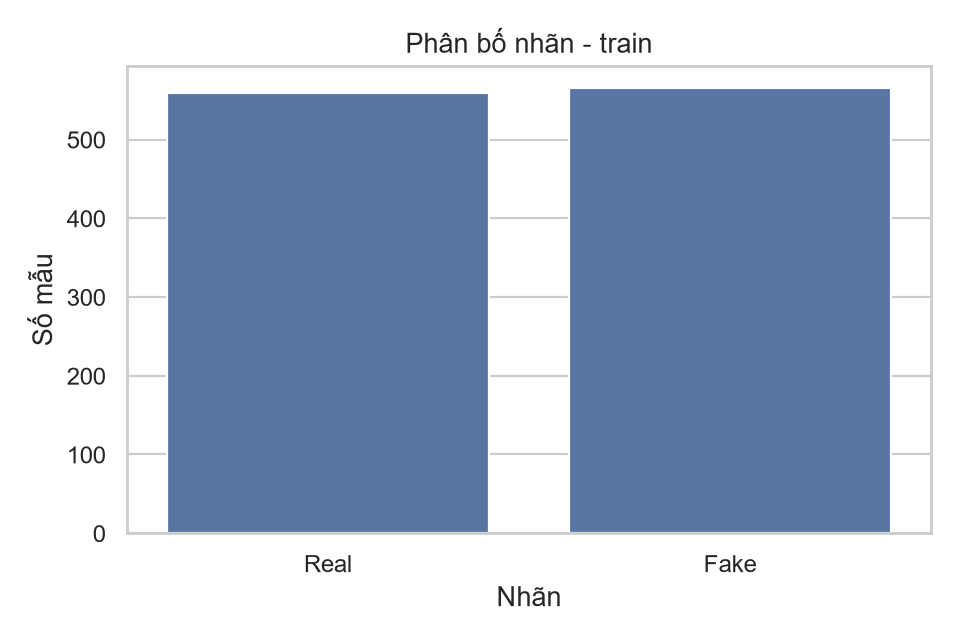
\includegraphics[width=0.75\textwidth]{figures/label_distribution.png}
\caption{Phân bố nhãn trong tập huấn luyện gốc}
\label{fig:labels}
\end{figure}

\begin{figure}[H]
\centering
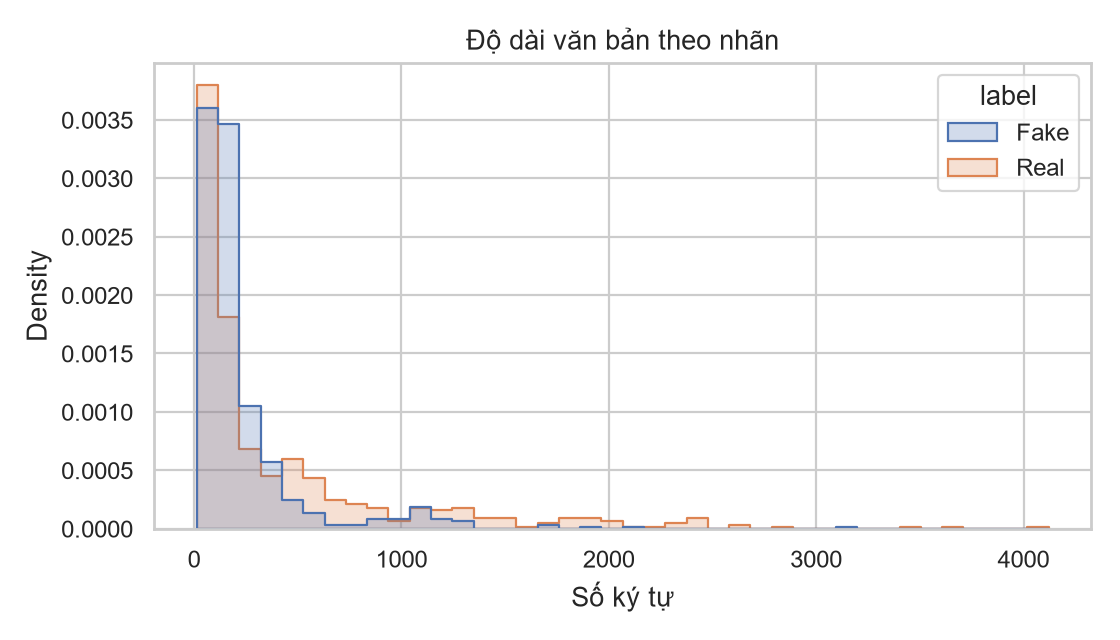
\includegraphics[width=0.85\textwidth]{figures/text_length.png}
\caption{Phân bố độ dài văn bản trong tập huấn luyện gốc}
\label{fig:length}
\end{figure}

\textit{Quy trình khử rò rỉ dữ liệu (Decontamination):} Quá trình kiểm tra phát hiện 136 mẫu trùng trong train, 9 mẫu trùng trong test và 64 văn bản trùng giao giữa hai tập. Kiểm tra đối chiếu xác nhận các mẫu này đều trùng khớp nguyên văn (exact string match) và bảo toàn qua phép chuẩn hóa chuỗi. Đặc biệt, toàn bộ 64 văn bản giao nhau này đều mang nhãn Fake. Nếu giữ nguyên, việc các mẫu này vừa xuất hiện trong train vừa có mặt trong test sẽ tạo ra hiện tượng rò rỉ dữ liệu nghiêm trọng, khiến mô hình chỉ cần ghi nhớ từ khóa là đạt điểm kiểm thử cao ảo ở lớp Fake. 

Nhóm áp dụng nguyên tắc làm sạch: \textbf{giữ lại bản ghi duy nhất trong tập kiểm thử độc lập và loại bỏ toàn bộ 64 văn bản trùng giao khỏi tập huấn luyện}. Tập huấn luyện sạch còn 924 mẫu (tỷ lệ Real/Fake là 559/365) và tập kiểm thử còn 273 mẫu duy nhất. Nội dung văn bản của tập kiểm thử chỉ được dùng để so khớp chuỗi nhằm khử trùng lặp; nhãn của tập kiểm thử hoàn toàn không được sử dụng trong bước chọn mô hình.

\section{Thiết kế thí nghiệm}
Tập huấn luyện sạch gồm 924 văn bản được phân chia theo phương pháp Stratified train/validation split với tỷ lệ 85\% huấn luyện (785 mẫu) và 15\% kiểm định (139 mẫu: 84 Real và 55 Fake) với hạt giống ngẫu nhiên cố định (\texttt{seed = 42}).

\begin{table}[H]
\centering
\caption{Cấu hình thực nghiệm các mô hình baseline}
\label{tab:cauhinh}
\begin{tabularx}{\textwidth}{p{3.5cm} X}
\toprule
\textbf{Thành phần} & \textbf{Thiết lập chi tiết} \\
\midrule
Trích xuất đặc trưng & TF--IDF, unigram và bigram cấp âm tiết, tối đa 100.000 đặc trưng, áp dụng sublinear TF scale, chuyển chữ thường \\
Phân chia kiểm định & Stratified split 85/15 trên 924 mẫu train sạch, seed = 42 \\
Majority Baseline & Dự đoán lớp đa số (DummyClassifier, strategy = most\_frequent) \\
Multinomial NB & Hệ số làm mịn cộng Laplace $\alpha = 0,5$ \\
Logistic Regression & Tối ưu hóa L-BFGS, $C = 2,0$, class\_weight = balanced, max\_iter = 2000 \\
Linear SVM & Dual linear formulation, $C = 1,0$, class\_weight = balanced \\
Tiêu chuẩn chọn mô hình & Macro-F1 cao nhất trên tập kiểm định validation \\
\bottomrule
\end{tabularx}
\end{table}

\section{Quy trình thực nghiệm}
Quy trình thực hiện tuần tự:
\begin{enumerate}[leftmargin=24pt]
  \item Nạp dữ liệu thô, chuẩn hóa khoảng trắng và ánh xạ nhãn chuẩn hóa về Real/Fake.
  \item Khám phá dữ liệu (EDA), phát hiện và loại bỏ các mẫu trùng lặp và văn bản giao nhau giữa hai tập.
  \item Chia tập huấn luyện sạch thành train/validation (85/15) theo phân bố nhãn.
  \item Huấn luyện và đánh giá chéo bốn mô hình baseline trong Sklearn Pipeline (đảm bảo vectorizer chỉ fit trên phần train của từng lượt).
  \item Lựa chọn mô hình có Macro-F1 validation cao nhất (Logistic Regression).
  \item Huấn luyện lại mô hình được chọn trên toàn bộ 924 mẫu train sạch.
  \item Đánh giá một lần duy nhất trên 273 mẫu kiểm thử độc lập; lưu trữ kết quả dự đoán và ma trận nhầm lẫn.
\end{enumerate}

% ----------------------------------------------------
% CHƯƠNG 5
% ----------------------------------------------------
\chapter{KẾT QUẢ THỰC NGHIỆM}

\section{Kết quả trên tập Validation}
Bảng~\ref{tab:validation} thể hiện kết quả so sánh bốn mô hình trên tập validation (139 mẫu).

\begin{table}[H]
\centering
\caption{Kết quả so sánh mô hình trên tập validation (N = 139 mẫu)}
\label{tab:validation}
\begin{tabular}{l rrrrr}
\toprule
\textbf{Mô hình} & \textbf{Accuracy} & \textbf{Macro-F1} & \textbf{Prec. Fake} & \textbf{Recall Fake} & \textbf{ROC--AUC} \\
\midrule
Majority Baseline & 0,6043 & 0,3767 & 0,0000 & 0,0000 & 0,5000 \\
Multinomial NB & 0,6978 & 0,5990 & \textbf{0,9333} & 0,2545 & 0,8879 \\
\textbf{Logistic Regression} & \textbf{0,8345} & \textbf{0,8226} & 0,8333 & \textbf{0,7273} & 0,8970 \\
Linear SVM & 0,8201 & 0,8056 & 0,8261 & 0,6909 & \textbf{0,9071} \\
\bottomrule
\end{tabular}
\end{table}

Logistic Regression đạt Macro-F1 = 0,8226, vượt Linear SVM (0,8056) và vượt trội so với Naive Bayes (0,5990) cũng như Majority Baseline (0,3767). Mặc dù Linear SVM có ROC--AUC nhỉnh hơn (0,9071 so với 0,8970), Logistic Regression được chọn do tiêu chí quyết định được cố định từ trước là Macro-F1.

\section{Đánh giá trên tập kiểm thử độc lập}
Mô hình Logistic Regression sau khi fit lại trên 924 mẫu train sạch được đánh giá trên 273 mẫu test duy nhất. Kết quả chi tiết được tổng hợp trong Bảng~\ref{tab:testmetrics}.

\begin{table}[H]
\centering
\caption{Các chỉ số đánh giá của Logistic Regression trên tập test sạch (N = 273)}
\label{tab:testmetrics}
\setlength{\tabcolsep}{4.5pt}
\begin{tabular}{rrrrrrrr}
\toprule
\textbf{Accuracy} & \textbf{Macro-P} & \textbf{Macro-R} & \textbf{Macro-F1} & \textbf{Fake-P} & \textbf{Fake-R} & \textbf{Fake-F1} & \textbf{ROC--AUC} \\
\midrule
\textbf{0,8535} & 0,8568 & 0,8506 & \textbf{0,8520} & 0,8803 & 0,7984 & 0,8374 & \textbf{0,9312} \\
\bottomrule
\end{tabular}
\end{table}

\begin{figure}[H]
\centering
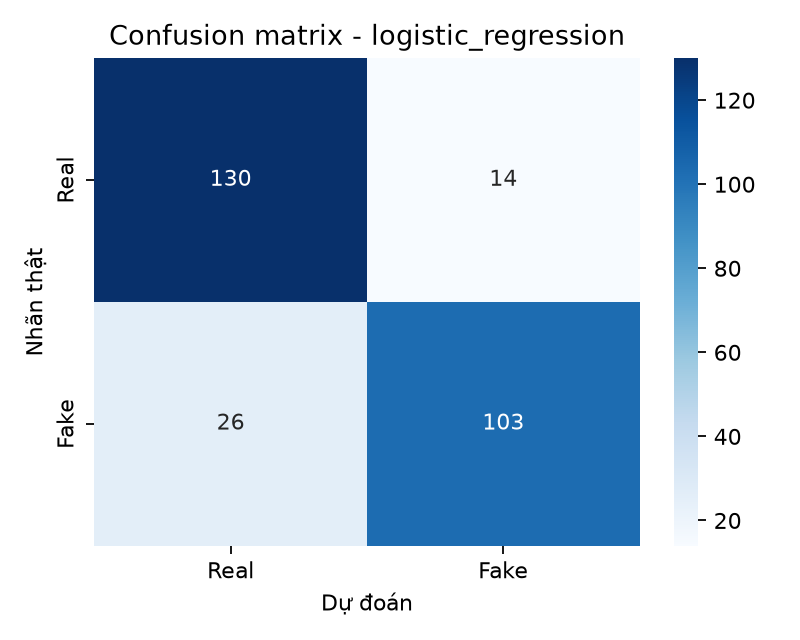
\includegraphics[width=0.6\textwidth]{figures/confusion_matrix.png}
\caption{Ma trận nhầm lẫn trên tập kiểm thử độc lập (Hàng: Nhãn thật, Cột: Dự đoán)}
\label{fig:cm}
\end{figure}

Ma trận nhầm lẫn (Hình~\ref{fig:cm}) chỉ ra rằng trong 273 mẫu kiểm thử:
\begin{itemize}[leftmargin=24pt]
  \item Lớp Real (144 mẫu): Dự đoán chính xác 130 mẫu (đạt Recall 90,28\%); dự đoán nhầm 14 mẫu thành Fake (False Positive).
  \item Lớp Fake (129 mẫu): Dự đoán chính xác 103 mẫu (đạt Recall 79,84\%); dự đoán nhầm 26 mẫu thành Real (False Negative).
\end{itemize}

\section{Phân tích lỗi và các trường hợp điển hình}
Tổng cộng có 40 trường hợp dự đoán sai (tỷ lệ lỗi 14,65\%). Thống kê độ dài văn bản của 40 mẫu dự đoán sai cho thấy: độ dài trung bình là 374,1 ký tự (độ lệch chuẩn 890,3 ký tự; biên độ từ 41 đến 5.350 ký tự; trung vị là 150 ký tự), trong khi nhóm dự đoán đúng có độ dài trung bình 299,7 ký tự.

Để hỗ trợ nhóm nghiên cứu rà soát trước khi bảo vệ, 6 mẫu dự đoán sai điển hình được trích xuất trực tiếp từ tệp \texttt{test\_predictions.csv} và đối chiếu khách quan:

\noindent\textbf{A. Nhóm Fake bị bỏ sót thành Real (26 trường hợp):}
\begin{itemize}[leftmargin=20pt]
  \item \textit{Mẫu 3 (191 ký tự):} ``sốc rơi cáp treo khiến 20 người tu vong tại chỗ sốc rơi cáp treo khiến 20 người tu vong tại chỗ...'' (lặp lại tiêu đề 4 lần). Nhãn tập dữ liệu: \textbf{Fake} $\rightarrow$ Mô hình dự đoán: \textbf{Real}.
  \item \textit{Mẫu 4 (150 ký tự):} ``bệnh bạch hầu có khả năng lây truyền nhanh và đáng sợ hơn covid19 người nhiễm bệnh có thể tử vong trong vòng 610 ngày nếu không được điều trị kịp thời''. Nhãn tập dữ liệu: \textbf{Fake} $\rightarrow$ Mô hình dự đoán: \textbf{Real}.
  \item \textit{Mẫu 38 (83 ký tự):} ``7 trường đại học ở việt nam ra trường dễ xin việc lọt top đại học tốt nhất thế giới''. Nhãn tập dữ liệu: \textbf{Fake} $\rightarrow$ Mô hình dự đoán: \textbf{Real}.
\end{itemize}

\noindent\textbf{B. Nhóm Real bị cảnh báo nhầm thành Fake (14 trường hợp):}
\begin{itemize}[leftmargin=20pt]
  \item \textit{Mẫu 36 (120 ký tự):} ``gấp gấp tìm người thân bà cụ đi lạc không nhớ nhà ai là người thân của cụ vui lòng gh công an xã tân thới nhì rước cụ về''. Nhãn tập dữ liệu: \textbf{Real} $\rightarrow$ Mô hình dự đoán: \textbf{Fake}.
  \item \textit{Mẫu 57 (249 ký tự):} ``tặng biên bản 75 triệu đồng cho người chị tung tin thất thiệt 1 nữ nhân viên samsung lây hiv cho 16 người tại thái nguyên phake cả danh sách...''. Nhãn tập dữ liệu: \textbf{Real} $\rightarrow$ Mô hình dự đoán: \textbf{Fake}. (Văn bản đưa tin chính thống về việc cơ quan chức năng xử phạt hành vi tung tin đồn giả, nhưng văn bản chứa nhiều từ ngữ nhạy cảm như ``tung tin thất thiệt'', ``phake'').
  \item \textit{Mẫu 65 (120 ký tự):} ``quá nguy hiểm xuất hiện trường hợp trộm đột nhập vào nhà không thèm cắt khóa bẻ khóa mà nhấc hẳn cửa ra khỏi bản lề luôn''. Nhãn tập dữ liệu: \textbf{Real} $\rightarrow$ Mô hình dự đoán: \textbf{Fake}.
\end{itemize}

\textit{Ghi chú quan trọng:} Các ví dụ trên được trích dẫn nhằm mô tả nội dung văn bản và nhãn dự đoán tương ứng trong tệp dữ liệu. Nhóm không đưa ra khẳng định suy diễn về nguyên nhân sai lệch khi chưa có phân tích định tính chuyên sâu độc lập. Nhóm cần rà soát lại các ca này trước buổi bảo vệ.

\section{Ứng dụng demo và giao diện dòng lệnh}
Hệ thống được đóng gói thành hai giao diện sử dụng:
\begin{enumerate}[leftmargin=24pt]
  \item \textbf{Giao diện Web Streamlit (\texttt{app/app.py}):} Cho phép người dùng nhập đoạn văn bản tiếng Việt và nhận về nhãn dự đoán kèm theo độ tin cậy ước lượng. Giao diện hiển thị khuyến cáo minh bạch: \textit{``Độ tin cậy ước lượng: 0.xxxx (xác suất mô hình (chưa hiệu chuẩn / uncalibrated))''} và lưu ý người dùng đây là kết quả học từ tập dữ liệu đóng, không thay thế kiểm chứng sự thật khách quan.
  \item \textbf{Giao diện dòng lệnh CLI (\texttt{src/project.py}):} Hỗ trợ lệnh dự đoán nhanh:
  \begin{center}
    \texttt{python -m src.project predict -{}-text "Nội dung cần kiểm tra"}
  \end{center}
  kèm cơ chế bắt lỗi an toàn khi nhập văn bản rỗng hoặc khi chưa huấn luyện mô hình.
\end{enumerate}

% ----------------------------------------------------
% CHƯƠNG 6
% ----------------------------------------------------
\chapter{KẾT LUẬN}

\section{Kết luận chính}
Trên bộ dữ liệu ViFN Version 1 sau khi đã xử lý triệt để rò rỉ dữ liệu trùng lặp, mô hình TF--IDF kết hợp Logistic Regression là mô hình tối ưu nhất trong các baseline được khảo sát, đạt Macro-F1 validation 0,8226 và Macro-F1 test 0,8520. Kết quả thực nghiệm đã xác nhận giả thuyết H1 và vượt mốc tham chiếu 0,70 được đặt ra trong H2.

\section{Trả lời các câu hỏi nghiên cứu}
\begin{itemize}[leftmargin=24pt]
  \item \textbf{Với RQ1:} Logistic Regression đạt Macro-F1 validation cao nhất (0,8226), vượt Linear SVM (0,8056), Multinomial Naive Bayes (0,5990) và Majority Baseline (0,3767).
  \item \textbf{Với RQ2:} Trên tập kiểm thử độc lập gồm 273 văn bản duy nhất, mô hình đạt Accuracy 0,8535; Macro-F1 0,8520 và ROC--AUC 0,9312. Tuy nhiên, Fake Recall chỉ đạt 0,7984 (bỏ sót 26/129 tin giả), cho thấy mô hình còn có xu hướng thiên về dự đoán lớp Real trong các trường hợp ranh giới.
\end{itemize}

\section{Giới hạn và hướng phát triển}
\textbf{Các giới hạn chính:}
\begin{enumerate}[leftmargin=24pt]
  \item \textbf{Quy mô corpus hạn chế:} Sau khi làm sạch, tập huấn luyện chỉ còn 924 mẫu và tập kiểm thử có 273 mẫu. Kích thước này chỉ đủ để đánh giá baseline cổ điển, chưa đủ lớn để đảm bảo độ tin cậy thống kê cao.
  \item \textbf{Nguy cơ rò rỉ ngữ nghĩa chưa được loại trừ hoàn toàn:} Phép khử trùng lặp chuỗi giải quyết được sự trùng lặp nguyên văn, nhưng chưa thể phát hiện các bài viết diễn đạt lại (paraphrase) hoặc đưa tin về cùng một sự kiện cụ thể. Mô hình có thể dựa vào các từ khóa phong cách nguồn thay vì bản chất sai lệch của thông tin.
  \item \textbf{Tokenization cấp âm tiết:} Việc chưa sử dụng công cụ phân đoạn từ tiếng Việt khiến mô hình bỏ lỡ các từ ghép đa âm tiết có ý nghĩa ngữ nghĩa chặt chẽ.
\end{enumerate}

\textbf{Hướng phát triển tiếp theo:}
\begin{itemize}[leftmargin=24pt]
  \item Thực hiện K-fold Stratified Cross-Validation lặp lại trên tập huấn luyện sạch để thu được khoảng tin cậy (confidence intervals) cho các độ đo.
  \item Tích hợp công cụ tách từ tiếng Việt chuẩn (\textit{pyvi} hoặc \textit{underthesea}) và thử nghiệm tinh chỉnh mô hình ngôn ngữ tiền huấn luyện (PhoBERT) khi có hạ tầng phần cứng GPU.
  \item Thu thập thêm siêu dữ liệu về nguồn xuất bản và mốc thời gian để đánh giá mô hình theo kịch bản chia tách miền (cross-domain) và chia tách thời gian (temporal split).
  \item Phát triển theo hướng Fact-checking dựa trên bằng chứng (Claim--Evidence) nhằm phục vụ bài toán kiểm chứng thông tin thực tế.
\end{itemize}

% ==================== TÀI LIỆU THAM KHẢO ====================
\clearpage
\chapter*{TÀI LIỆU THAM KHẢO}
\addcontentsline{toc}{chapter}{TÀI LIỆU THAM KHẢO}

\begin{enumerate}[label={[\arabic*]}, leftmargin=24pt]
  \bibitem{huynh2025utilizing}
  A.-T. Huynh và P. Tran, ``Utilizing Transformer Models to Detect Vietnamese Fake News on Social Media Platforms,'' \textit{KSII Transactions on Internet and Information Systems}, vol. 19, no. 2, pp. 472--487, 2025. DOI: \url{https://doi.org/10.3837/tiis.2025.02.006}.

  \bibitem{scikit_tfidf}
  Scikit-learn developers, ``TfidfVectorizer,'' tài liệu thư viện scikit-learn. Truy cập tại: \url{https://scikit-learn.org/stable/modules/generated/sklearn.feature_extraction.text.TfidfVectorizer.html}.

  \bibitem{scikit_lr}
  Scikit-learn developers, ``LogisticRegression,'' tài liệu thư viện scikit-learn. Truy cập tại: \url{https://scikit-learn.org/stable/modules/generated/sklearn.linear_model.LogisticRegression.html}.

  \bibitem{scikit_nb}
  Scikit-learn developers, ``MultinomialNB,'' tài liệu thư viện scikit-learn. Truy cập tại: \url{https://scikit-learn.org/stable/modules/generated/sklearn.naive_bayes.MultinomialNB.html}.

  \bibitem{scikit_svm}
  Scikit-learn developers, ``LinearSVC,'' tài liệu thư viện scikit-learn. Truy cập tại: \url{https://scikit-learn.org/stable/modules/generated/sklearn.svm.LinearSVC.html}.

  \bibitem{tran2025vifactcheck}
  T. H. Tran, Q. D. Tran, K. Q. Tran và K. V. Nguyen, ``ViFactCheck: A New Benchmark Dataset and Methods for Multi-Domain News Fact-Checking in Vietnamese,'' trong \textit{Proceedings of the AAAI Conference on Artificial Intelligence}, vol. 39, no. 1, 2025. DOI: \url{https://doi.org/10.1609/aaai.v39i1.32008}.

  \bibitem{vifn2025github}
  Huynh Tuan, ``ViFN -- Vietnamese Fake News Datasets Version 1,'' kho lưu trữ GitHub chính thức. Truy cập tại: \url{https://github.com/huynhtuan0106/ViFN-Vietnamese_Fake_New_Datasets_Ver1}.
\end{enumerate}

% ==================== PHỤ LỤC ====================
\clearpage
\appendix
\chapter{HƯỚNG DẪN TÁI LẬP THỰC NGHIỆM}

Phần này hướng dẫn các bước cài đặt và chạy lại toàn bộ thí nghiệm trên máy tính cá nhân chạy hệ điều hành Windows:

\section*{Bước 1: Thiết lập môi trường thực thi}
Mở cửa sổ Windows PowerShell tại thư mục gốc của dự án:
\begin{verbatim}
py -3.11 -m venv .venv
.\.venv\Scripts\Activate.ps1
python -m pip install --upgrade pip
pip install -r requirements.txt
\end{verbatim}

\section*{Bước 2: Chuẩn bị dữ liệu}
Tải hai tệp \texttt{train\_data.csv} và \texttt{test\_data.csv} từ kho lưu trữ GitHub chính thức của ViFN Version 1 và lưu tại:
\begin{verbatim}
data/raw/train_data.csv
data/raw/test_data.csv
\end{verbatim}

\section*{Bước 3: Chạy phân tích khám phá dữ liệu (EDA)}
Thực hiện lệnh:
\begin{verbatim}
python -m src.project eda
\end{verbatim}
Lệnh này sẽ tính toán thống kê mô tả, kiểm tra trùng lặp và lưu trữ kết quả tại \texttt{outputs/metrics/eda\_summary.json} cùng hai biểu đồ trong \texttt{outputs/figures/}.

\section*{Bước 4: Huấn luyện và đánh giá mô hình}
Thực hiện lệnh:
\begin{verbatim}
python -m src.project train
\end{verbatim}
Lệnh sẽ tự động thực hiện khử trùng lặp rò rỉ, chia validation 85/15, so sánh 4 baseline, chọn mô hình theo Macro-F1, huấn luyện lại trên toàn bộ 924 mẫu sạch, đánh giá trên 273 mẫu test sạch và lưu mô hình tối ưu tại \texttt{models/best\_model.joblib}.

\section*{Bước 5: Chạy dự đoán dòng lệnh hoặc ứng dụng web}
Dự đoán nhanh một câu tin tức qua dòng lệnh:
\begin{verbatim}
python -m src.project predict --text "Nội dung tin tức cần kiểm tra"
\end{verbatim}

Khởi chạy ứng dụng giao diện trực quan Streamlit:
\begin{verbatim}
streamlit run app/app.py
\end{verbatim}

\end{document}

